\subsection{Artifically Intelligent Agents}
    It is generally accepted that an artificial intelligence needs to possess the qualities shown in Figure \ref{fig:AIcapabilities} \cite{Russell2010-wv,Nilsson2009-rp,Luger2008-vf}\footnote{This group of capabilities would generally be accepted in the AI community, although it may be necessary to add other categories like imagination, creativity, and social interaction. Of course this set of attributes is not universally accepted, and is still being refined.}. However, the following simple definitions will help to ground further discussion in the paper:

    \begin{description}
        \item [Reasoning (R)]: The ability to solve problems, and make conclusions.
        \item [Knowledge Representation (K)]: The ability to internally represent knowledge of information that has been learned.
        \item [Planning (Pl)]: The ability to make a plan in order to accomplish a goal within an environment.
        \item [Learning (L)]: The ability to learn from experience and data.
        \item [Perception (Pe)]: The ability to use different sensors to perceive the surrounding environment.
        \item [Motion/Manipulation (M)]: The ability to move within an environment and manipulate parts of it.
        \item [Interaction (I)]: The ability to interact with other intelligent agents. For communicating with humans this could involve some type of natural language interface.
    \end{description}

	\begin{figure}[htbp]
    	\centering
     	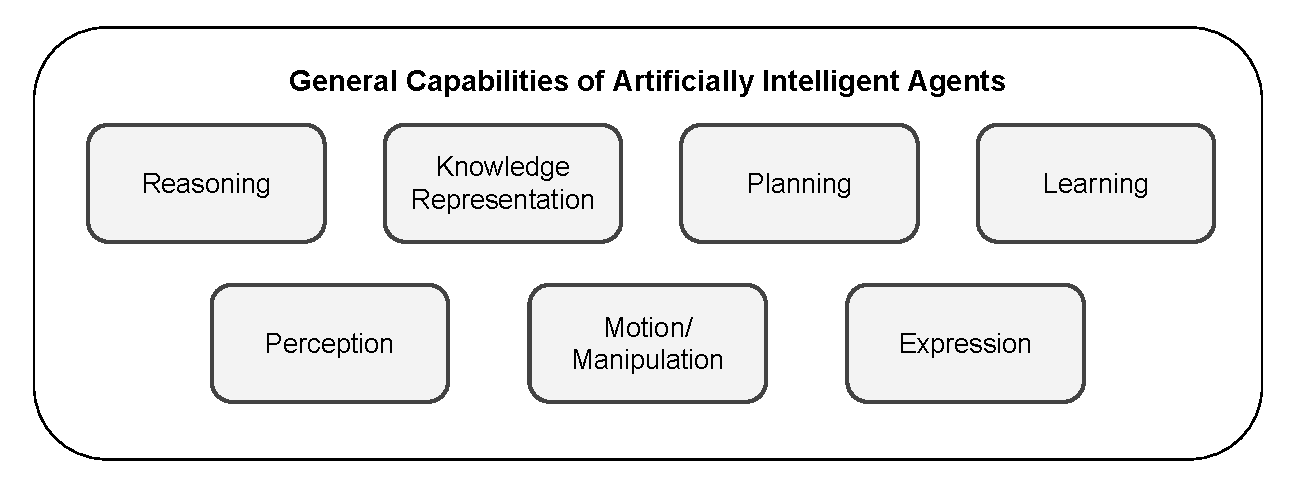
\includegraphics[width=0.7\textwidth]{Figures/AI_capabilities}
    	\caption{List of the capabilities of an artificial general intelligence. In this paper an AI is defined as a system that possesses at least one of the capabilities illustrated.}
        \label{fig:AIcapabilities}
    \end{figure}

    As noted by \cite{Tripp2011-cq} technology spans a wide spectrum of capabilities. With regards to autonomous systems one might consider anything from a thermostat, to a Tesla autopilot. While most of the current focus is geared towards our capability to trust `advanced` technology, for the purposes of this survey I wish to take a more holistic view and use the term Artificially Intelligent Agent (AIA) to encompass a broad range of technologies that can be considered automatic by some sense of the word.

    It should be noted that the categories are not clearly separable; for instance where does the capability to plan end, and reasoning begin? Similar questions could be asked of the other capabilities. Regardless, given this set of capabilities an AIA can then be defined as:
    
    \begin{description}
        \item[Artificially Intelligent Agent:] an agent that possess, to some extent, at least one of the capabilities shown in the figure \ref{fig:AIcapabilities}. 
    \end{description}

    Arguably I might just use the term AI instead of AIA. However, the term AI carries too much ambiguity. Using the term AIA allows me to broadly include ***any*** system in the weak-strong/ narrow-broad plane. Figure \ref{fig:StrongWeak} shows some examples of AIAs and their places on the plane.

    One might also question the need to define AIAs in the first place. This is to aid in the search for assurances. As will be shown later, assurances span the range of AIAs so that an automation system might be able to use similar assurances to a self-driving car, and vice-versa. 

    This definition while \emph{extremely} broad is still useful because it encompasses many of the systems that are currently being marketed as ``artificially intelligent'' at this time. More importantly, many of the assurances that exist for the simplest AIA (e.g. a simple classifier) can be extended for use in more advanced AIAs. In other words, using the proposed definition of an AIA sets the appropriate scope for research that is likely to contain assurances that apply to AIAs.

    In order to help ground the discussion Figure \ref{fig:StrongWeak} shows several AIA systems on a coordingate system of 

	\begin{figure}[htbp]
    	\centering
     	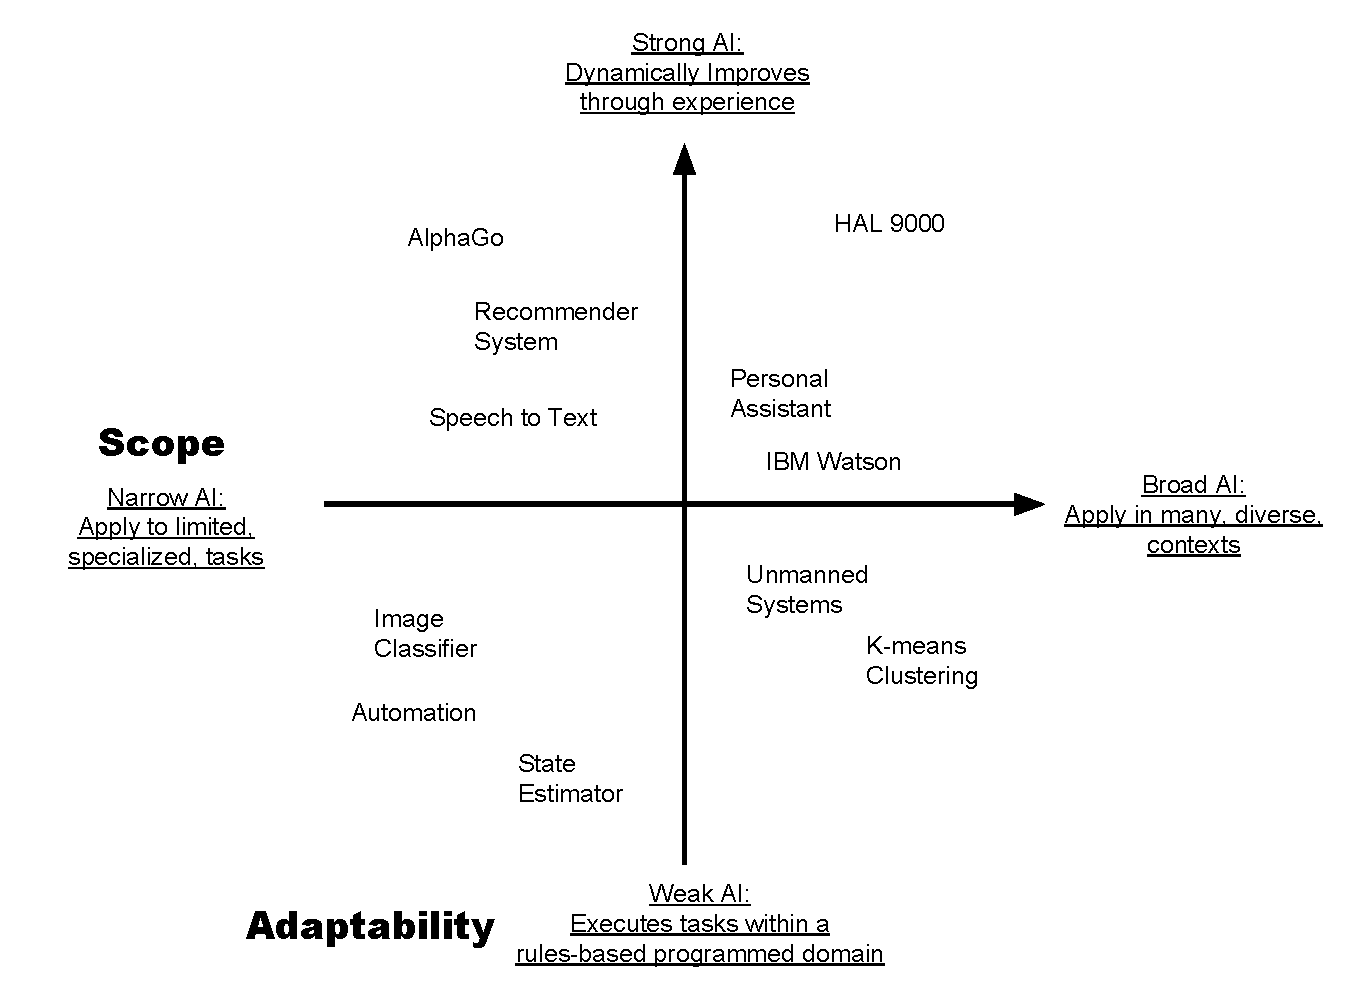
\includegraphics[width=0.7\textwidth]{Figures/strong_weak_narrow_broad.pdf}
    	\caption{Illustration of the range of systems encompassed by the AIA definition. Horizontal axis reflects the scope of the AIA, the vertical axis reflects the adaptability of the AIA.}
        \label{fig:StrongWeak}
    \end{figure}

    To make sure the point is clear, the research discipline called machine learning (ML) is a subset of the AI research landscape. Individual ML algorithms might be thought of as being a narrowly scoped AI that is contained within only one of the AGI capabilities. Concretely, the following systems currently exist and may possess the listed AIA capabilities.
    
    \begin{enumerate}
         \item An autonomous bottle capping machine might perceive bottles, and perform movements to place a cap on them
         \item An unmanned aerial system (UAS) might possess the ability to plan missions, perceive its location, and act to accomplish that plan
         \item A virtual personal assistant might be capable of interacting with a user, learn the user's preferences, and reason about what assistance the user needs
         \item An image classifier might possess the capability to learn image classes from labeled examples and predict the class of never-before-seen new images.
     \end{enumerate}

     The definition of AIA and understanding of the range of capabilities helps to understand what kinds of assurances might be needed. For example an assurance from an AIA that can plan will probably differ in design and/or application from that of an AIA that can perceive.
